\section{Results}\label{sec:results}
Table~\ref{tab:main-results} gives the two stored primary endpoints
without pooling their populations. The original computation completed
all 456 instances, retaining 11592 accepted and 7560 incompatible measured
observations with no numerical or external-accuracy rejection. Its
168 paired observations yield \OriginalEstimate\% median relative
reduction, with 95\% limits \OriginalLower\% and \OriginalUpper\%.
Figure~\ref{fig:original-effect} displays this interval and the
registered ten-percent reference. The interval crosses zero, so the
original prediction is unestablished. The result is not replaced by
the best-performing dimension or a selected repetition.
\begin{table}[htbp]\centering\footnotesize
\caption{Distinct primary populations, stored effect estimates and uncertainty for the two completed timing studies. Failed-pair rules are not transferred between experiments and neither registered ten percent improvement criterion is established.}\label{tab:main-results}
\begin{tabularx}{\textwidth}{@{}>{\raggedright\arraybackslash}Xrrrr@{}}\toprule
Study & Population & Pairs & Effect (\%) & 95\% limits\\\midrule
Separable & 456 & 168 & 0.\allowbreak{}499839 & -3.\allowbreak{}29197, 3.\allowbreak{}94484\\
Grouped & 210 & 144 & -212.\allowbreak{}45 & -225.\allowbreak{}337, -192.\allowbreak{}874\\
\bottomrule\end{tabularx}
\end{table}

\begin{figure}[htbp]\centering
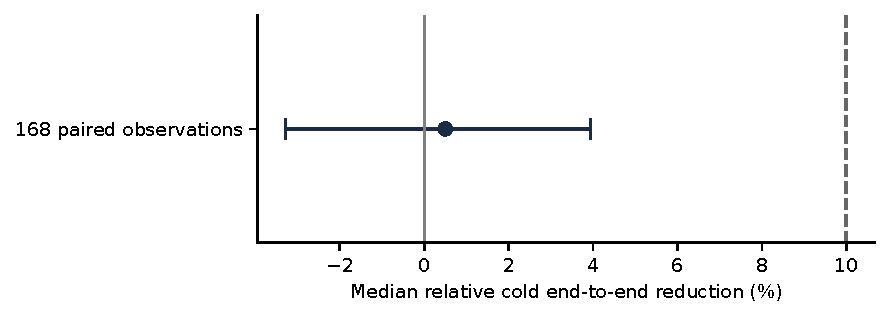
\includegraphics[width=.94\textwidth]{figures/original-effect.pdf}
\caption{Original held-out timing estimate with its stored 95 percent seed-cluster confidence interval and registered ten percent reference. The interval crosses zero; neither interval nor population is recomputed for this figure.}\label{fig:original-effect}
\end{figure}


Figure~\ref{fig:scalar-objective} relates the original scalar objective
to the actual returned method optima. Agreement outside the preferred
interval is consistent with the declared finite departure price.
The analytic curve is an evaluation of stored coefficients, not
another timed trial. Figure~\ref{fig:cold-times} instead displays
stored cell medians and interquartile ranges in one asymmetric-elastic
slice. It shows concrete complete-call costs while retaining its
descriptive status. Formulation size and a selected timing curve
cannot establish a general factorization or algorithmic advantage.
\begin{figure}[htbp]\centering
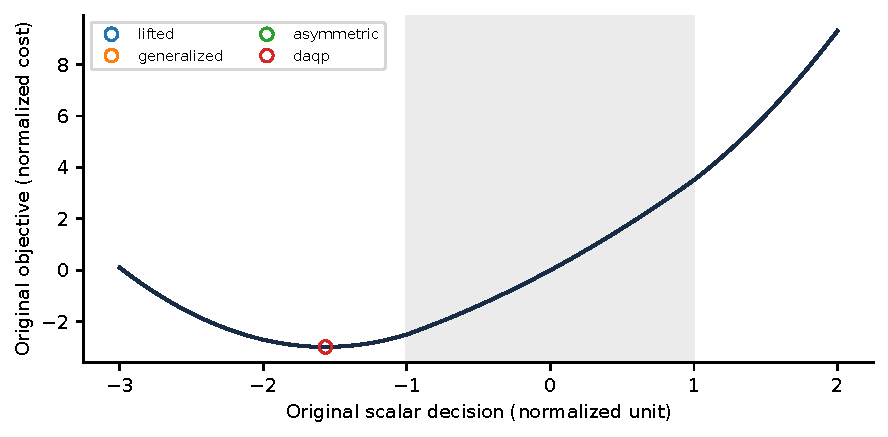
\includegraphics[width=.94\textwidth]{figures/scalar-objective.pdf}
\caption{Analytic evaluation of the stored C01 objective and actual exported method optima. The shaded interval is the preferred band, and the curve is a mathematical illustration rather than a new timed observation.}\label{fig:scalar-objective}
\end{figure}

\begin{figure}[htbp]\centering
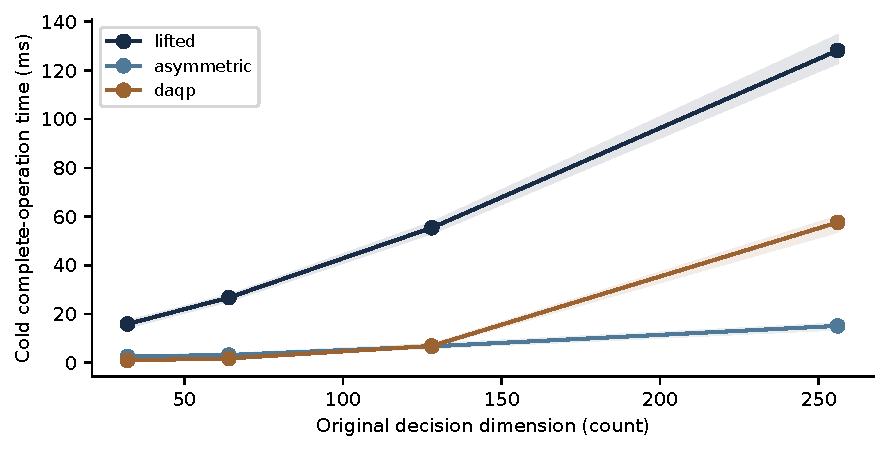
\includegraphics[width=.94\textwidth]{figures/cold-times.pdf}
\caption{Stored held-out asymmetric-elastic timing cells at density 0.05 and unit diagonal condition. Lines are stored medians and bands stored interquartile ranges; this descriptive subset does not replace the complete primary endpoint.}\label{fig:cold-times}
\end{figure}


The original conditioning comparison in
Figure~\ref{fig:conditioning} retains the maximum accepted objective
discrepancy for each compatible robustness cell. The finite grid
extends through diagonal condition$10^6$ without violating the
registered objective/hard limits in admitted observations. This is
not a proof for every near-dependent or arbitrarily scaled problem.
The common-trajectory stream in Figure~\ref{fig:stream-reuse} shows
stored cold and warm durations; it has one observation per frame
and does not support an independent statistical superiority claim.
Its component interpretation is examined in the next section.
\begin{figure}[htbp]\centering
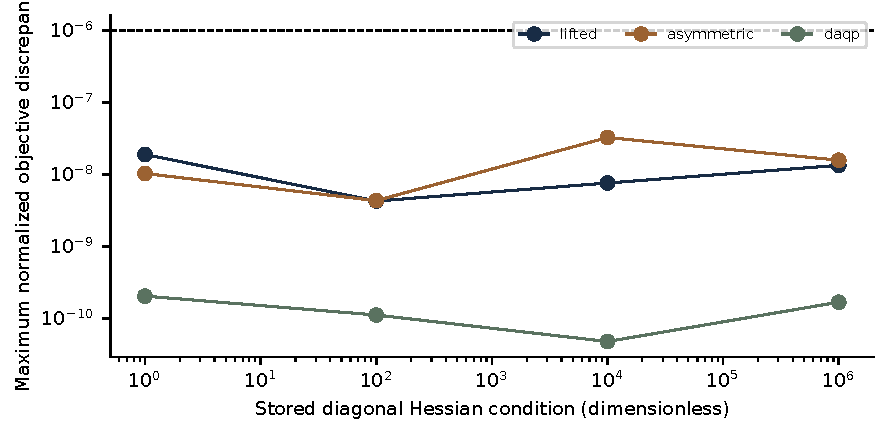
\includegraphics[width=.94\textwidth]{figures/conditioning.pdf}
\caption{Maximum stored objective discrepancy in each compatible robustness cell by diagonal condition. The dashed line is the original external objective criterion; absent methods remain absent rather than receiving an invented zero discrepancy.}\label{fig:conditioning}
\end{figure}

\begin{figure}[htbp]\centering
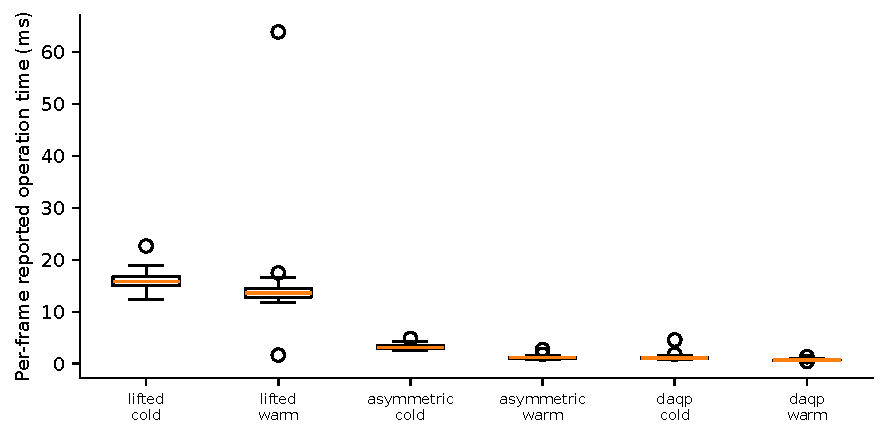
\includegraphics[width=.94\textwidth]{figures/stream-reuse.pdf}
\caption{Stored cold and warm C12 operation durations for every accepted frame of each compatible method. The box summaries are descriptive paired-path evidence, not a randomized causal isolation of warm starting from all other implementation choices.}\label{fig:stream-reuse}
\end{figure}


The grouped study completed all 210 canonical inputs. Its 5670 measured
method observations comprise 3667 accepted,12 accuracy-rejected,
1719 incompatible,270 dependent oracle-failed and two supervised
timeouts. Table~\ref{tab:coupled-states} and
Figure~\ref{fig:coupled-states} retain those categories separately
in development, held-out and robustness splits. The 7770 raw
observations additionally retain warm-ups and oracle calls. All
163390 returned candidate frames satisfy the applicable original-
space checks;44 noncandidate backend-limit frames remain distinct.
Framewise mathematical agreement does not override a failed operation's
batch-level state or the primary failed-pair treatment.
\begin{table}[htbp]\centering\footnotesize
\caption{Measured grouped-study method states by split, including dependent oracle failures and supervised timeouts. Counts cover all measured method rows, while warm-up and oracle observations remain in the larger raw archive.}\label{tab:coupled-states}
\begin{tabularx}{\textwidth}{@{}>{\raggedright\arraybackslash}Xrrrrr@{}}\toprule
Split & Accepted & Accuracy & Incompat. & Oracle & Timeout\\\midrule
development & 879 & 0 & 396 & 21 & 0\\
heldout & 2587 & 6 & 1188 & 105 & 2\\
robustness & 201 & 6 & 135 & 144 & 0\\
\bottomrule\end{tabularx}
\end{table}

\begin{figure}[htbp]\centering
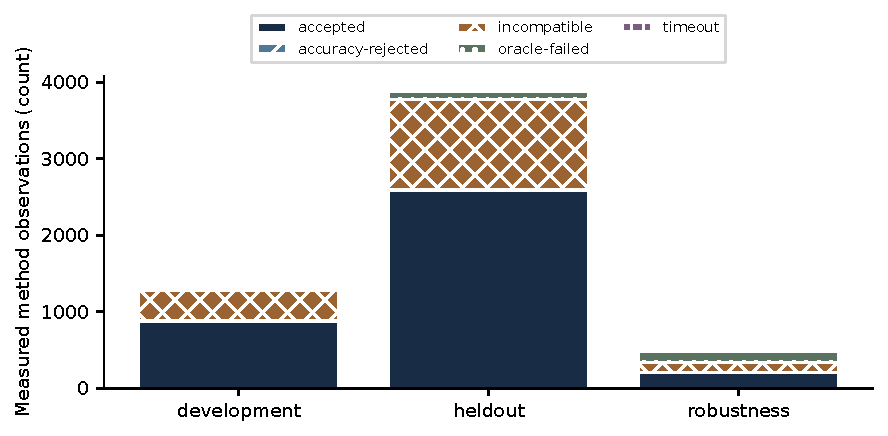
\includegraphics[width=.94\textwidth]{figures/coupled-states.pdf}
\caption{All 5670 measured method observations of the grouped study, separated by their original development, held-out and robustness splits. Acceptance, accuracy rejection, incompatibility, dependent oracle failure and supervised timeout remain different categories.}\label{fig:coupled-states}
\end{figure}


The complete 144-member grouped endpoint is shown in
Figure~\ref{fig:coupled-population}. Nine failed pairs retain their
prespecified score; six missing native medians remain gaps. No
reference is selected where the primary rule selected none.
The median paired score is \PrimaryEstimate\%, with 95\% limits
\PrimaryLower\% and \PrimaryUpper\%. These percentages do not
describe a uniform slowdown of every instance, and the result
does not become favorable by discarding unsuccessful members.
Figure~\ref{fig:coupled-formulations} shows returned per-instance
method medians with their differing sample counts. Those unmatched
distributions characterize concrete formulations but are not an
alternative primary estimator.
\begin{figure}[htbp]\centering
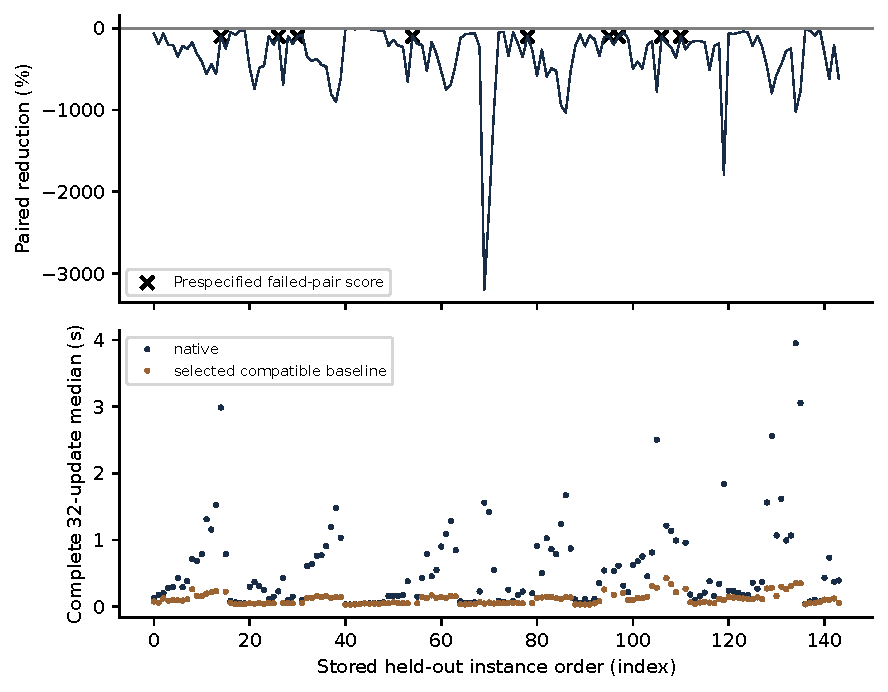
\includegraphics[width=.94\textwidth]{figures/coupled-population.pdf}
\caption{All 144 stored grouped-study primary members in original order, with nine failed scores retained. Complete-operation medians preserve missing values as gaps and do not impute a comparator where the primary rule selected none.}\label{fig:coupled-population}
\end{figure}

\begin{figure}[htbp]\centering
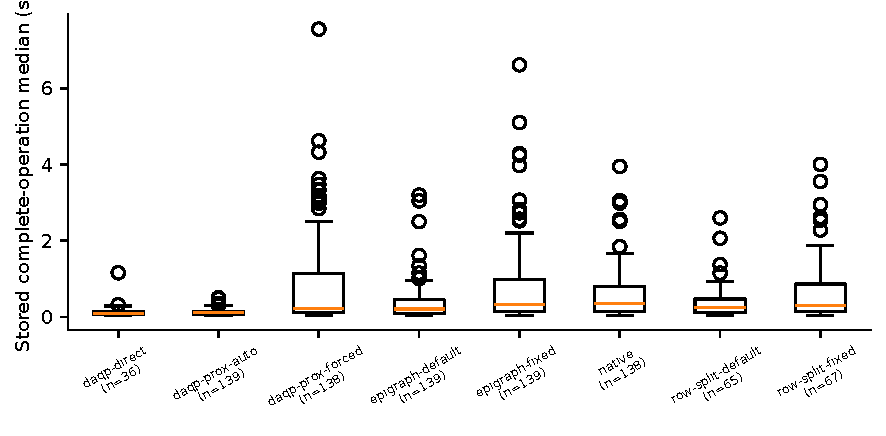
\includegraphics[width=.94\textwidth]{figures/coupled-formulations.pdf}
\caption{Distributions of stored held-out per-instance medians for each returned compatible formulation. Sample counts differ because compatibility and failures differ; these unmatched descriptive distributions are not the registered paired comparison or a causal ablation.}\label{fig:coupled-formulations}
\end{figure}


Figure~\ref{fig:directional-lesson} supplies a transparent original-
space agreement example from the stored physical teaching input.
Native, compact-epigraph and directional row-split answers agree
on objective and decision within their numerical criteria. The
example supports the intended formulation equivalence; it adds
no timed observation to either registered population. Its role
is to separate a mathematical or implementation correctness claim
from the computational hypothesis that the full studies refute.
Thus the results are consistent: exact proximal identities and
small accepted examples coexist with negative complete-operation
timing findings on the specified tested populations.
\begin{figure}[htbp]\centering
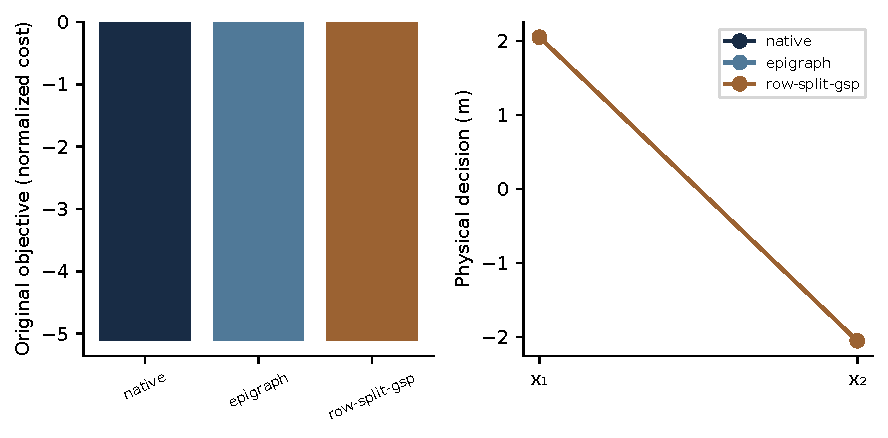
\includegraphics[width=.94\textwidth]{figures/directional-lesson.pdf}
\caption{Stored native, epigraph and directional row-split answers for the same two-variable physical teaching input. Objective and decision agreement are a small numerical illustration, not additional timing evidence or an independent experiment.}\label{fig:directional-lesson}
\end{figure}

The twelve accuracy-rejected batches include backend or iteration-limit
and absent-vector outcomes, rather than twelve returned vectors failing
the independent KKT calculation. Six held-out row-split batches returned
status seven without a candidate vector. Native and forced-proximal DAQP
operations account for the two timeouts. Six robustness oracle limits
leave 144 dependent measured rows with oracle-failed state in that split.
Those dependency counts are distinct from the nine failed primary pairs.
All returned candidate frames passed their applicable original-space
checks; a batch-level backend status remains a separate acceptance condition.
